%% DONE
\newpage
\let\cleardoublepage\clearpage
\part{Производственные и обрабатывающие отрасли}
\chapter{Пищевая технология}
\ID{IRSTI 65.59.31}{}

\begin{articleheader}
\sectionwithauthors{Sh.B. Baitukenova, U.A. Ryspaeva, S.B. Baitukenova}{DEVELOPMENT OF FERMENTED SAUSAGE PRODUCTION TECHNOLOGY USING STARTER CULTURES OF MICROORGANISMS}

{\bfseries
\textsuperscript{2}Sh.B. Baitukenova\textsuperscript{\envelope } \authorid,
\textsuperscript{1}U.A. Ryspaeva\authorid,
\textsuperscript{1}S.B. Baitukenova\authorid}
\end{articleheader}

\begin{affiliation}
\emph{\textsuperscript{1}JSC «Kazakh University of Technology and
Business named after K. Kulazhanov», Astana, Kazakhstan,}

\emph{\textsuperscript{2}NAO «Kazakh Agrotechnical Research University
named after S.Seifullin», Astana, Kazakhstan}

\raggedright {\bfseries \textsuperscript{\envelope }}{\em Сorresponding author: \href{mailto:baytukenova75@mail.ru}{\nolinkurl{baytukenova75@mail.ru}}}
\end{affiliation}

This article considers the influence of microorganisms on the
composition of semi-smoked sausages and technological processes. Liquid
propionic acid bacteria were introduced into beef and their biological
value, organoleptic and physicochemical parameters were studied. The
influence of the use of starter microorganisms on tenderness, juiciness,
nutritional value of the finished product, formation of the necessary
level of structure and ability to retain moisture was studied, and also
it was established that due to the action of starter microorganisms
organoleptic indicators increase. As a result of experimental samples
and researches the optimised formulation and technology of fermented
semi-smoked sausages have been created.

Physico-chemical, organoleptic indicators, moisture-holding capacity,
active acidity pH of the finished product and raw materials were
determined. The method of production of fermented semi-smoked sausages
is characterised by the introduction of starter culture into the raw
material after the stage of meat grinding, before salting. The optimal
ratio of liquid propionibacterium Propionibacterium shermani and
Lactobacillus acidophilus, L.casei, L.Plantarum (2 strains of
propionibacterium shermani and Lactobacillus acidophilus) is 0.1\%,
fermentation time - 8 hours.

Based on the results of experimental studies, we consider the use of
liquid propionic acid bacteria `ProBioLiz' (2 strains of propionic acid
bacteria Propionibacterium shermani and lactobacillus).

{\bfseries Keywords:} 1st and 2nd category beef, starter microorganisms,
propionic acid microorganism, fermented beef, fermented half-sausages,
amino acid composition.

\begin{articleheader}
{\bfseries СТАРТЕР МИКРОАҒЗАЛАРЫМЕН ӨҢДЕЛГЕН ФЕРМЕНТТЕЛГЕН ЖАРТЫЛАЙ
ЫСТАЛҒАН ШҰЖЫҚ ЖАСАУ ТЕХНОЛОГИЯСЫН ӘЗІРЛЕУ}

{\bfseries \textsuperscript{2}Ш.Б. Байтукенова\textsuperscript{\envelope },
\textsuperscript{1}У.А. Рыспаева, \textsuperscript{1}С.Б. Байтукенова}
\end{articleheader}

\begin{affiliation}
\emph{\textsuperscript{1}«Қ.Құлажанов атындағы Қазақ технология және
бизнес университеті» АҚ, Астана, Қазақстан,}

\emph{\textsuperscript{2}«С.Сейфуллин атындағы Қазақ агротехникалық
зерттеу университеті», Астана, Қазақстан,}

\emph{e-mail: \href{mailto:baytukenova75@mail.ru}{\nolinkurl{baytukenova75@mail.ru}}}
\end{affiliation}

Бұл мақалада микроорганизмдердің жартылай ысталған шұжықтардың құрамына
және технологиялық процестеріне әсері қарастырылады. Сиыр етіне сұйық
пропион қышқылы бактериялары қосылып, олардың биологиялық құндылығы,
органолептикалық және физика-химиялық көрсеткіштері зерттелді.
Стартерлік микроорганизмдерді қолданудың дайын өнімнің нәзіктігіне,
шырындылығына, тағамдық құндылығына, құрылымның қажетті деңгейінің
қалыптасуына және ылғалды сақтау қабілетіне әсері зерттелді, сонымен
қатар әрекетке байланысты стартердің органолептикалық көрсеткіштері
жоғарылайды екендігі анықталды. Эксперименттік үлгілер мен зерттеулер
нәтижесінде ферменттелген жартылай ысталған шұжықтардың оңтайландырылған
рецептісі мен технологиясы жасалды.

Дайын өнім мен шикізаттың физикалық-химиялық, органолептикалық
көрсеткіштері, ылғал ұстау қабілеті, белсенді қышқылдығының рН-ы
анықталды. Ферменттелген жартылай ысталған шұжықтарды өндіру әдісі етті
ұсақтау кезеңінен кейін, тұздаудың алдында шикізатқа стартерлі
микроағзаны енгізумен сипатталады. «ProBioLys» сұйық пропион қышқылы
бактериясын (Propionibacterium shermani және lactobacilli Lactobacillus
acidophilus, L.casei, L.Plantarum пропион қышқылының 2 штаммы)
пайдаланудың оңтайлы арақатынасы 0,1\%, ферменттеу уақыты 8 сағат.

Эксперименттік зерттеулердің нәтижелеріне сүйене отырып, ысталған ет
өнімдерінде сұйық пропион қышқылы бактериясы «ProBioLys»
(Propionibacterium shermani және lactobacilli Lactobacillus acidophilus,
L.casei, L.Plantarum пропион қышқылының 2 штаммы) сұйық пропион қышқылы
бактериясын қолдану орынды деп санаймыз.

{\bfseries Түйін сөздер:} 1 және 2 санаттағы сиыр еті, бастапқы
микроорганизмдер, пропион қышқылы микроорганизмі, ферменттелген сиыр
еті, ферменттелген жартылай шұжықтар, аминқышқыл құрамы.

\begin{articleheader}
{\bfseries РАЗРАБОТКА ТЕХНОЛОГИИ ПРОИЗВОДСТВА ФЕРМЕНТИРОВАННОЙ КОЛБАСЫ С
ПРИМЕНЕНИЕМ СТАРТОВЫХ КУЛЬТУР МИКРООРГАНИЗМОВ}

{\bfseries \textsuperscript{2}Ш.Б. Байтукенова\textsuperscript{\envelope },
\textsuperscript{1}У.А. Рыспаева, \textsuperscript{1}С.Б. Байтукенова}
\end{articleheader}

\begin{affiliation}
\emph{\textsuperscript{1}АО «Казахский университет технологии и бизнеса
имени К. Кулажанова», Астана, Казахстан,}

\emph{\textsuperscript{2} НАО «Казахский агротехнический
исследовательский университет им. С.Сейфуллина», Астана, Казахстан,}

\emph{e-mail:
\href{mailto:baytukenova75@mail.ru}{\nolinkurl{baytukenova75@mail.ru}}}
\end{affiliation}

В данной статье рассмотрено влияние микроорганизмов на состав
полукопченых колбас и технологические процессы. В говядину вносили
жидкие пропионокислые бактерии и изучали их биологическую ценность,
органолептические и физико-химические показатели. Изучено влияние
использования заквасочных микроорганизмов на нежность, сочность, пищевую
ценность готового продукта, формирование необходимого уровня структуры и
способность удерживать влагу, а также установлено, что за счет действия
закваски повышаются органолептические показатели. В результате
экспериментальных образцов и исследований создана оптимизированная
рецептура и технология ферментированных полукопченых колбас.

Определены физико-химические, органолептические показатели,
влагоудерживающая способность, рН активной кислотности готового продукта
и сырья. Способ производства ферментированных полукопченых колбас
характеризуется введением в сырье стартовую культуру после стадии
измельчения мяса, перед посолом. Оптимальное соотношение использования
жидкой пропионовокислой бактерии «ПроБиоЛиз» (2 штамма пропионовокислой
бактерии Propionibacterium shermani и лактобациллы Lactobacillus
acidophilus, L.casei, L.Plantarum) составляет 0,1\%, время ферментации
-- 8 часов.

На основании результатов экспериментальных исследований мы считаем
актуальным использование жидкой пропионовокислой бактерии «ПроБиоЛиз» (2
штамма пропионовокислой бактерии Propionibacterium shermani и
лактобактерий Lactobacillus acidophilus, L.casei, L.Plantarum) в
копченых мясных продуктах.

{\bfseries Ключевые слова:} говядина 1-й и 2-й категории, стартовые
микроорганизмы, пропионовокислый микроорганизм, ферментированная
говядина, ферментированные полуколбасы, аминокилотный состав.

\begin{multicols}{2}
{\bfseries Introduction.} The most important condition for increasing the
range of sausage products is to reduce the cost of sausage products
while maintaining standard quality. Currently, the best way to solve
this problem is the introduction of new technologies that improve the
biochemical changes occurring during the processing of meat raw
materials. The use of microorganisms in the production of meat products
helps to improve the quality of the finished product {[}1{]}.

Currently, there are many large-scale theoretical and experimental
materials on the use of sourdough starters in sausage production,
including the study of probiotic microorganisms of scientific interest.
Probiotic microorganisms include bifido and propionic acid bacteria.
Propionic acid bacteria grow at low temperatures, produce odorous,
antimutagenic substances, vitamin B12, amino acids, and are highly
active against pathogenic microflora.

Fermented sausages are produced at a constant temperature and, depending
on the relative humidity, depending on the change in microbiological,
biochemical and physical processes during ripening.

During the ripening of sausages, proteins are broken down into
oligopeptides and free amino acids by the formation of histenzyme and
aminopeptidase, which has a very good effect on the flavour of the
finished product {[}2{]}.

The aim of the work was to study the biochemical activity of propionic
acid bacteria at the stage after treatment of raw materials with starter
microorganisms at the stages of the technological process of production
of semi-smoked sausages.

Propionic acid and bifidobacteria are very widely used in food
production. Therefore, it is important to determine the odour-correcting
and biochemical activity of the bacteria. In the works of Khanhalaev
I.A. and I.S. Khamagaeva the influence of propionic acid and
bifidobacteria on the finished sausage product was considered and it was
proved that organoleptic parameters are significantly improved {[}3{]}.

In their work, P. Nedelsheva and D. Zenkova proved that the addition of
probiotic strain Lactobacillus Plantarum to the raw material provides
mass and reduction of pathogenic flora in raw smoked sausage due to the
necessary fermentation process {[}4{]}.

In their workM. Laranjo and M.E. Potes suggested that propionic acid
bacteria increase the safety of fermented meat products by rapidly
acidifying the matrix and producing antimicrobial agents such as
bacteriocins {[}5{]}.

In his works S.E. Shokesheva, Y.M. Uzakov studied the effect of starter
microorganisms on the acceleration of ripening of finished meat products
and microstructure of finished sausage {[}6{]}.

{\bfseries Materials and methods.} Scientific and experimental work was
carried out in the experimental shop for processing of meat products. As
a material for experiments were taken experimental samples of
semi-smoked sausage made on the basis of standard GOST 31785-2012. ST RK
1731-2007 Determination of organoleptic quality indicators of meat and
meat products was carried out.

Acidity pH and water activity in sausage was measured using a digital
pH-meter. The sample was chopped and mixed by passing it twice through a
meat grinder. The prepared solution (1:10 ratio with distilled water)
was determined from the mixture obtained after settling at 20°C for 30
minutes. The study was repeated 5 times. The total value is obtained
from the method of variance calculation.

The ability to bind moisture was determined by the pressing method,
based on the separation of water from the test sample during pressing,
sorption of the separated moisture with filter paper and determination
of the amount of water. The study was carried out by repeating 5 times
by the area of the spot left on the filter paper. The total value is
obtained based on the method of variance calculation.

Counting the number of mesophilic aerobic and facultative-anaerobic
microorganisms in the prepared samples and the number of colonies in
Petri dishes was carried out in accordance with ST GOST R 51448-2010 of
the Republic of Kazakhstan. This study was carried out after the
manufacture of samples and after expiry date.

Liquid propionic acid bacteria `ProBioLyz' (2 strains of propionic acid
bacteria Propionibacterium shermani and lactobacillus Lactobacillus
acidophilus, L.casei, L.Plantarum) 0.08\%, 0.1\%, 0.15\% per 100 kg were
used as a starter.

The technological process was carried out in accordance with the
technological instructions in compliance with the rules for meat
industry enterprises.

The method of production of fermented semi-smoked sausages was
characterised by the introduction of starter microorganisms into the raw
material after the stage of meat grinding, before salting. Beef
semi-smoked sausage was chosen as the basic recipe (Table 1).
\end{multicols}

\begin{table}[H]
\caption*{Table 1 - Recipe for fermented semi-smoked sausage}
\centering
\begin{tabular}{|l|l|lll|}
\hline
\multirow{2}{*}{Raw materials}    & \multirow{2}{*}{Beef sausage} & \multicolumn{3}{c|}{100 кг/кг}                                           \\ \cline{3-5} 
                                  &                               & \multicolumn{1}{l|}{Sample 1} & \multicolumn{1}{l|}{Sample 2} & Sample 3 \\ \hline
beef 1 grade                      & 85                            & \multicolumn{1}{l|}{60}       & \multicolumn{1}{l|}{55}       & 50       \\ \hline
beef 2 grade                      & -                             & \multicolumn{1}{l|}{25}       & \multicolumn{1}{l|}{30}       & 35       \\ \hline
Raw fat                           & 10                            & \multicolumn{1}{l|}{10}       & \multicolumn{1}{l|}{10}       & 10       \\ \hline
Egg powder                        & 5                             & \multicolumn{1}{l|}{5}        & \multicolumn{1}{l|}{5}        & 5        \\ \hline
Total quantity:                   & 100,00                        & \multicolumn{1}{l|}{100,00}   & \multicolumn{1}{l|}{100,00}   & 100,00   \\ \hline
\textbf{Spices:}                  &                               & \multicolumn{1}{l|}{}         & \multicolumn{1}{l|}{}         &          \\ \hline
Table salt                        & 2,5                           & \multicolumn{1}{l|}{2,5}      & \multicolumn{1}{l|}{2,5}      & 2,5      \\ \hline
Icing sugar                       & 1,0                           & \multicolumn{1}{l|}{1,0}      & \multicolumn{1}{l|}{1,0}      & 1,0      \\ \hline
Black pepper                      & 0,8                           & \multicolumn{1}{l|}{0,8}      & \multicolumn{1}{l|}{0,8}      & 0,8      \\ \hline
Sodium nitrite                    & 0,045                         & \multicolumn{1}{l|}{0,040}    & \multicolumn{1}{l|}{0,030}    & 0,025    \\ \hline
Starter microorganism ‘PROBIOLIS’ & -                             & \multicolumn{1}{l|}{0,08}     & \multicolumn{1}{l|}{0,1}      & 0,15     \\ \hline
\end{tabular}
\end{table}

{\bfseries Results and discussion}: According to the results of chemical
analysis, it can be seen that the protein content and mineral
composition of the new fermented sausage product is not significantly
higher than that of the exemplary sausages (Table 2).

\begin{table}[H]
\caption*{Table 2 - Chemical composition of fermented semi-smoked sausage product}
\centering
\begin{tabular}{|l|llll|}
\hline
\multirow{2}{*}{Indicators}              & \multicolumn{4}{c|}{Half-smoked sausage}                                                                                                                                                                                       \\ \cline{2-5} 
                                         & \multicolumn{1}{l|}{‘Beef’ (sample)} & \multicolumn{1}{p{0.15\textwidth}|}{Fermented semi-smoked sausage (test sample 1)} & \multicolumn{1}{p{0.15\textwidth}|}{Fermented semi-smoked sausage (test sample 2)} & \multicolumn{1}{p{0.15\textwidth}|}{Fermented semi-smoked sausage (test sample 3)} \\ \hline
Mass fraction of moisture, \%            & \multicolumn{1}{c|}{64,3±0,53}       & \multicolumn{1}{c|}{65,5±0,3}                                      & \multicolumn{1}{c|}{65,3±0,6}                                      & 65,5±0,5                                      \\ \hline
Mass fraction of protein, \%             & \multicolumn{1}{c|}{11,40±0,2}       & \multicolumn{1}{c|}{11,6±0,3}                                      & \multicolumn{1}{c|}{11,60±0,2}                                     & 11,60±0,3                                     \\ \hline
Mass fraction of fat, \%                 & \multicolumn{1}{c|}{21,10±0,2}       & \multicolumn{1}{c|}{21,58±0,2}                                     & \multicolumn{1}{c|}{21,58±0,23}                                    & 21,58±0,2                                     \\ \hline
Acidity, pH                              & \multicolumn{1}{c|}{5,9±0,02}        & \multicolumn{1}{c|}{5,3±0,01}                                      & \multicolumn{1}{c|}{5,5±0,01}                                      & 5,5±0,02                                      \\ \hline
\multicolumn{1}{|p{0.25\textwidth}|}{Mass fraction of residual sodium nitrite} & \multicolumn{1}{c|}{0,06±0,0002}     & \multicolumn{1}{c|}{0,0025±0,0002}                                 & \multicolumn{1}{c|}{0,0033±0,0002}                                 & 0,002±0,0001                                  \\ \hline
\end{tabular}
\end{table}

\begin{multicols}{2}
It can also be seen that the mass fraction of moisture in the samples
slightly increased and the acidity significantly decreased. And residual
sodium nitrite in the tested sample was reduced compared to the control
sample. The decrease in residual sodium nitrite in the tested samples
was due to the action of starter microorganisms.

The rapid change in the transformation and colour formation of sodium
nitrite can be attributed to the decrease in acidity of pH. Due to the
reduction of residual sodium nitrite, a saturated colour of the finished
product can be obtained.

According to the results of the amino acid composition analysis, it can
be seen that the protein of the sample is significantly richer in amino
acids than the amino acids contained in the semi-smoked sausage `Beef'.
An increase in tryptophan, lysine, isoleucine, valine, leucine,
threonine was observed in fermented semi-smoked sausage (Table 3).
\end{multicols}

\begin{table}[H]
\caption{Table 3 - Amino acid composition of semi-smoked sausage}
\centering
\begin{tabular}{|l|cccc|}
\hline
\multirow{3}{*}{Amino acids} & \multicolumn{2}{c|}{Quantity, 1 mg per 100g}                                                                                     & \multicolumn{2}{c|}{Amino acid value, \%}                                                                                                                                             \\ \cline{2-5} 
                             & \multicolumn{4}{c|}{Half-smoked sausage}                                                                                                                                                                                                                                                                                 \\ \cline{2-5} 
                             & \multicolumn{1}{l|}{‘Beef’ (sample)} & \multicolumn{1}{l|}{\begin{tabular}[c]{@{}l@{}}Fermented sausage\\  (trial)\end{tabular}} & \multicolumn{1}{l|}{\begin{tabular}[c]{@{}l@{}}Fermented sausage\\  (trial)\end{tabular}} & \multicolumn{1}{l|}{\begin{tabular}[c]{@{}l@{}}Fermented sausage\\  (trial)\end{tabular}} \\ \hline
                             & \multicolumn{1}{c|}{836,454}         & \multicolumn{1}{c|}{907,023}                                                              & \multicolumn{1}{c|}{170}                                                                  & 184                                                                                       \\ \hline
Valine                       & \multicolumn{1}{c|}{572,678}         & \multicolumn{1}{c|}{701,096}                                                              & \multicolumn{1}{c|}{124}                                                                  & 140                                                                                       \\ \hline
Isoleucine                   & \multicolumn{1}{c|}{1036,987}        & \multicolumn{1}{c|}{1336,084}                                                             & \multicolumn{1}{c|}{112}                                                                  & 132                                                                                       \\ \hline
Leucine                      & \multicolumn{1}{c|}{1025,999}        & \multicolumn{1}{c|}{1383,846}                                                             & \multicolumn{1}{c|}{155}                                                                  & 184                                                                                       \\ \hline
Lysine                       & \multicolumn{1}{c|}{367,654}         & \multicolumn{1}{c|}{411,613}                                                              & \multicolumn{1}{c|}{88}                                                                   & 84                                                                                        \\ \hline
Methionine                   & \multicolumn{1}{c|}{571,033}         & \multicolumn{1}{c|}{705,714}                                                              & \multicolumn{1}{c|}{132}                                                                  & 150                                                                                       \\ \hline
Threonine                    & \multicolumn{1}{c|}{169,031}         & \multicolumn{1}{c|}{187,023}                                                              & \multicolumn{1}{c|}{112}                                                                  & 128                                                                                       \\ \hline
Tryptophan                   & \multicolumn{1}{c|}{497,987}         & \multicolumn{1}{c|}{676,682}                                                              & \multicolumn{1}{c|}{70}                                                                   & 78                                                                                        \\ \hline
Phenylalaline                & \multicolumn{1}{c|}{5077,823}        & \multicolumn{1}{c|}{6309,081}                                                             & \multicolumn{1}{c|}{120}                                                                  & 130                                                                                       \\ \hline
\end{tabular}
\end{table}

\begin{multicols}{2}
The amount of substituted amino acids does not tend to fluctuate
strongly. That is why the content of amino acids in the sour sausage
semi-smoked is higher than in the sample. From the above results,
comparing the sample with the test sample, it is clear that the amount
of essential amino acids methonine in the test sample is lower by 0.4
mg/g protein, in the test sample phenylalanine increased by 0.8 mg/g
protein

Biological value of the finished product is determined by the
composition of mineral substances and vitamins. An important indicator
of the nutritional value of fats is the acid composition of fat. It
increases the flavour and energy value of the finished product. Minerals
and vitamins play an important role in the human body. The human body
cannot synthesise vitamins, so they enter the human body through
products of plant and animal origin. Deficiency of vitamins and minerals
in food leads to metabolic disorders in the human body {[}7{]}.

Table 4 shows the amount of minerals and vitamins in fermented
semi-smoked sausage.
\end{multicols}

\begin{table}[H]
\caption*{Table 4 - Mineral substances and vitamins in fermented semi-smoked sausages}
\centering
\begin{tabular}{|lcccc|}
\hline
\multicolumn{1}{|l|}{Indicators, 100 mg}      & \multicolumn{1}{l|}{‘Beef’ (sample)} & \multicolumn{1}{p{0.15\textwidth}|}{Fermented semi-smoked sausage (test sample 1)} & \multicolumn{1}{p{0.15\textwidth}|}{Fermented semi-smoked sausage (test sample 2)} & \multicolumn{1}{p{0.15\textwidth}|}{Fermented semi-smoked sausage (test sample 3)} \\ \hline
\multicolumn{5}{|l|}{Minerals:}                                                                                                                                                                                                                                                                     \\ \hline
\multicolumn{1}{|l|}{Calcium (Ca)}            & \multicolumn{1}{c|}{34,12±3,65}      & \multicolumn{1}{c|}{34,51±5}                                       & \multicolumn{1}{c|}{34,50±6,9}                                     & 34,50±5,5                                                          \\ \hline
\multicolumn{1}{|l|}{Magnesium (Mg)}          & \multicolumn{1}{c|}{5,61±1,07}       & \multicolumn{1}{c|}{5,73±1,1}                                      & \multicolumn{1}{c|}{5,70±1,14}                                     & 5,73±1,2                                                           \\ \hline
\multicolumn{1}{|l|}{iron (Fe)}               & \multicolumn{1}{c|}{1,77±0,3}        & \multicolumn{1}{c|}{1,85±0,5}                                      & \multicolumn{1}{c|}{1,85±0,37}                                     & 1,87±0,43                                                          \\ \hline
\multicolumn{5}{|l|}{Vitamins:}                                                                                                                                                                                                                                                                     \\ \hline
\multicolumn{1}{|l|}{Retinol (A)}             & \multicolumn{1}{c|}{0,018}           & \multicolumn{1}{c|}{0,031}                                         & \multicolumn{1}{c|}{0,027}                                         & 0,03                                                               \\ \hline
\multicolumn{1}{|l|}{Tocopherol (E)}          & \multicolumn{1}{c|}{0,027}           & \multicolumn{1}{c|}{0,039}                                         & \multicolumn{1}{c|}{0,031}                                         & 0,04                                                               \\ \hline
\multicolumn{1}{|l|}{Ascorbic acid (C)}       & \multicolumn{1}{c|}{0,41}            & \multicolumn{1}{c|}{0,42}                                          & \multicolumn{1}{c|}{0,43}                                          & 0,42                                                               \\ \hline
\multicolumn{1}{|l|}{Niacin PP}               & \multicolumn{1}{c|}{2,63}            & \multicolumn{1}{c|}{2,71}                                          & \multicolumn{1}{c|}{2,65}                                          & 2,71                                                               \\ \hline
\multicolumn{1}{|l|}{Thiamine (B1)}           & \multicolumn{1}{c|}{0,19}            & \multicolumn{1}{c|}{0,2}                                           & \multicolumn{1}{c|}{0,25}                                          & 0,2                                                                \\ \hline
\multicolumn{1}{|l|}{Riboflavin (B2)}         & \multicolumn{1}{c|}{0,2}             & \multicolumn{1}{c|}{0,22}                                          & \multicolumn{1}{c|}{0,21}                                          & 0,22                                                               \\ \hline
\multicolumn{1}{|l|}{Energy value, kcal (kJ)} & \multicolumn{1}{c|}{244,7 (1023,8)}  & \multicolumn{1}{c|}{250,5 (1048,09)}                               & \multicolumn{1}{c|}{250,5 (1048,09)}                               & 250,5 (1048,09)                                                    \\ \hline
\end{tabular}
\end{table}

\begin{multicols}{2}
According to biological sciences, fats, minerals are not only explained
by substances and vitamins, the quality of their individual components
is determined, as well as the presence of individual amino acids in
protein and the presence of semi-unsaturated fatty acids in fats. The
rate of digestion of protein in the intestinal structure or digestion of
food by proteolytic enzymes is one of the important factors determining
the biological value of food.

We investigated fermented semi-smoked sausages taking into account that
the biological value of protein, which depends on the quantitative units
of amino acids, is degraded by enzymes. In a sample of specifically
fermented semi-smoked sausage, a hydrolysis stage due to starter
microorganisms was observed.

In conclusion, having analysed the research data, we are convinced that
the starter has an optimal effect on the biological parameters and food
quality of the finished product. By treating meat raw material with
propionic acid microorganism, it is possible to increase the species,
physical and chemical composition, biological value of the finished
product. Thus, we can conclude that propionic acid microorganisms
developing in minced meat lead to a significant increase in the content
of non-exchangeable amino acids in raw meat.

In order to evaluate the effect of fermented raw materials on the
properties of the finished product, a study of such indicators as
moisture-holding capacity, active acidity, and yield of the finished
product was carried out (Table 5).
\end{multicols}

\begin{table}[H]
\caption*{Table 5 - Physico-chemical parameters of a sample of semi-smoked sausage}
\centering
\begin{tabular}{|l|cccc|}
\hline
\multirow{2}{*}{Indicators}                        & \multicolumn{4}{c|}{Finished product}                                                                                                                                                                                                                 \\ \cline{2-5} 
                                                   & \multicolumn{1}{l|}{Beef sausage} & \multicolumn{1}{l|}{Sample 1 100 kg/kg} & \multicolumn{1}{l|}{\begin{tabular}[c]{@{}l@{}}Sample 2\\  100 кг/кг\end{tabular}} & \multicolumn{1}{l|}{\begin{tabular}[c]{@{}l@{}}Sample 3\\  100 кг/кг\end{tabular}} \\ \hline
Active acidity, pH                                 & \multicolumn{1}{c|}{5,9}          & \multicolumn{1}{c|}{5,5}                & \multicolumn{1}{c|}{5,3}                                                           & 5,5                                                                                \\ \hline
\multicolumn{1}{|p{0.2\textwidth}|}{Moisture retention capacity, by product weight, \%} & \multicolumn{1}{c|}{60}           & \multicolumn{1}{c|}{60,9}               & \multicolumn{1}{c|}{62.3}                                                          & 63,8                                                                               \\ \hline
Finished product yield, \%                         & \multicolumn{1}{c|}{103,5}        & \multicolumn{1}{c|}{104,4}              & \multicolumn{1}{c|}{105,8}                                                         & 106                                                                                \\ \hline
\end{tabular}
\end{table}

\begin{multicols}{2}
Looking at the values in Table 5, it can be seen that the active acidity
of the experimental sausages is lower than the pH value of the control
sample. It is very important to evaluate the pH value (active acidity)
of meat raw material for sausage production.

Analysing the obtained data, it can be said that the strains of selected
microorganisms grow in the minced meat sample, which can be judged by
the accumulation of lactic acid and decrease in the pH of the medium.

The increase in lactic acids during meat fermentation led to a decrease
in pH (active acid), thereby increasing the resistance of raw materials
to putrefactive microorganisms, increasing connective tissue collagen,
and changing the odour and flavour of meat.

The decomposition of carbohydrates and organic acids after treatment of
raw materials with the starter microorganism showed that the
accumulation of lactic acid resulted in a significantly higher rate of
acidification in treated batches than in the control, which is in
agreement with the report of Lin and Zhang {[}8{]}.

One of the most important indicators of sausage products is moisture
retention and binding integrity. The importance of water in the
production of meat and meat products is very important for the
production and storage of products. Moisture affects the yield of the
product due to the softness of the finished product, loss of mass during
heat treatment.

The starter culture has a very high moisture content, processing of raw
material leads to changes in the internal structure of meat, our goal is
to control the change in moisture content of prototypes after processing
of raw material with culture.

The aim of the study was to determine the quality of the finished
product, pH-activity, concentration of organic acids, microbiological
quality and organoleptic suitability of semi-smoked sausage with the
addition of liquid propionic acid bacteria starter `ProBioLiz' (2
strains were observed propionic acid bacteria Propionibacterium shermani
and lactobacilli Lactobacillus acidophilus, L.casei, L.Plantarum).

Taking into account the biological value, organoleptic and
physico-chemical indicators of the finished product, it is recommended
to use fermented beef for the production of semi-smoked sausage. The
optimal ratio of using liquid propionic acid bacteria `ProBioLiz' (2
strains of propionic acid bacteria Propionibacterium shermani and
lactobacillus Lactobacillus acidophilus, L.casei, L.Plantarum) is 0.1\%,
fermentation time - 8 hours.

Table 5 shows that the control sample of non-fermented minced meat under
study has lower moisture binding capacity than the fermented minced meat
samples. From the data obtained, it can be seen that there is a tendency
to increase the moisture-binding capacity of the sausage sample with the
addition of experimental cultures.

The ability of raw materials to retain moisture is characterised by the
ability of raw materials to retain moisture during thermal processing.
This indicator ensures the yield of the finished product and is the most
important technological indicator. Because the yield of the finished
product increases with the increase of moisture holding capacity.

Based on the studies of some authors, such as Marcel Mati, M. Magal, J.
Karovicova, Ladislav Staruch, it is proved that when meat products are
treated with starter microorganisms, moisture retention increases by
0.96 \% {[}9{]}.

After 2 hours of culturing the sample with 0.1\% starter in the finished
product, the lactic acid content increased by 5.5\% compared to the
control. After 6 hours, the difference was 15.3\%, indicating a faster
accumulation of lactic acid in the sample. This allows to increase
moisture retention properties, due to which the content of active acid
decreases.

Microbiological indicators of sausages, namely the number of mesophilic
aerobic and facultative-anaerobic microorganisms, were taken into
account in two stages - after sausages preparation and after the expiry
of storage period. The results were processed in accordance with TR TS
TS 034/2013 `On the safety of meat and meat products' {[}10{]}.
\end{multicols}

\begin{table}[H]
\caption*{Table 6 - Microbiological parameters of semi-smoked sausage after smoking}
\centering
\begin{tabular}{|l|l|l|l|l|l|}
\hline
On request                                                           & \begin{tabular}[c]{@{}l@{}}СU TR\\  034/2013\end{tabular} & Beef sausage & Sample 1 100 kg/kg & \begin{tabular}[c]{@{}l@{}}Sample 2\\  100 кг/кг\end{tabular} & \begin{tabular}[c]{@{}l@{}}Sample 3\\  100 кг/кг\end{tabular} \\ \hline
\begin{tabular}[c]{@{}l@{}}NoMAaAM\\   CFU*/g, not more\end{tabular} & Not allowed                                               & unavailable  & unavailable        & unavailable                                                   & 1*$10^2$ , не менее                                              \\ \hline
\begin{tabular}[c]{@{}l@{}}Yeast\\  CFU*/g, not more\end{tabular}    & 100                                                       & 10           & 20                 & 50                                                            & 120                                                           \\ \hline
\end{tabular}
\end{table}

\begin{table}[H]
\caption*{Table 7 - Microbiological indices of semi-smoked sausage after expiry date of sausage products}
\centering
\begin{tabular}{|l|c|c|c|c|c|}
\hline
On request                                                           & \multicolumn{1}{l|}{\begin{tabular}[c]{@{}l@{}}СU TR\\  034/2013\end{tabular}} & \multicolumn{1}{l|}{Beef sausage} & \multicolumn{1}{l|}{Sample 1 100 kg/kg} & \multicolumn{1}{l|}{\begin{tabular}[c]{@{}l@{}}Sample 2\\  100 кг/кг\end{tabular}} & \multicolumn{1}{l|}{\begin{tabular}[c]{@{}l@{}}Sample 3\\  100 кг/кг\end{tabular}} \\ \hline
\begin{tabular}[c]{@{}l@{}}NoMAaAM\\   CFU*/g, not more\end{tabular} & 1*$10^4$ & 1*$10^8$ & 1*$10^5$ & 1*$10^4$ & 1*$10^2$                                                                              \\ \hline
\begin{tabular}[c]{@{}l@{}}Yeast\\  CFU*/g, not more\end{tabular}    & 100                                                                            & 30                                & 45                                      & 80                                                                                 & 150                                                                                \\ \hline
\end{tabular}
\end{table}

\begin{figure}[H]
	\centering
	
\includegraphics[width=0.6\columnwidth]{media/pish/image1}
	\caption*{Figure 1 - Organoleptic evaluation of semi-smoked sausages using propionic acid bacteria}
\end{figure}

\begin{figure}[H]
	\centering
	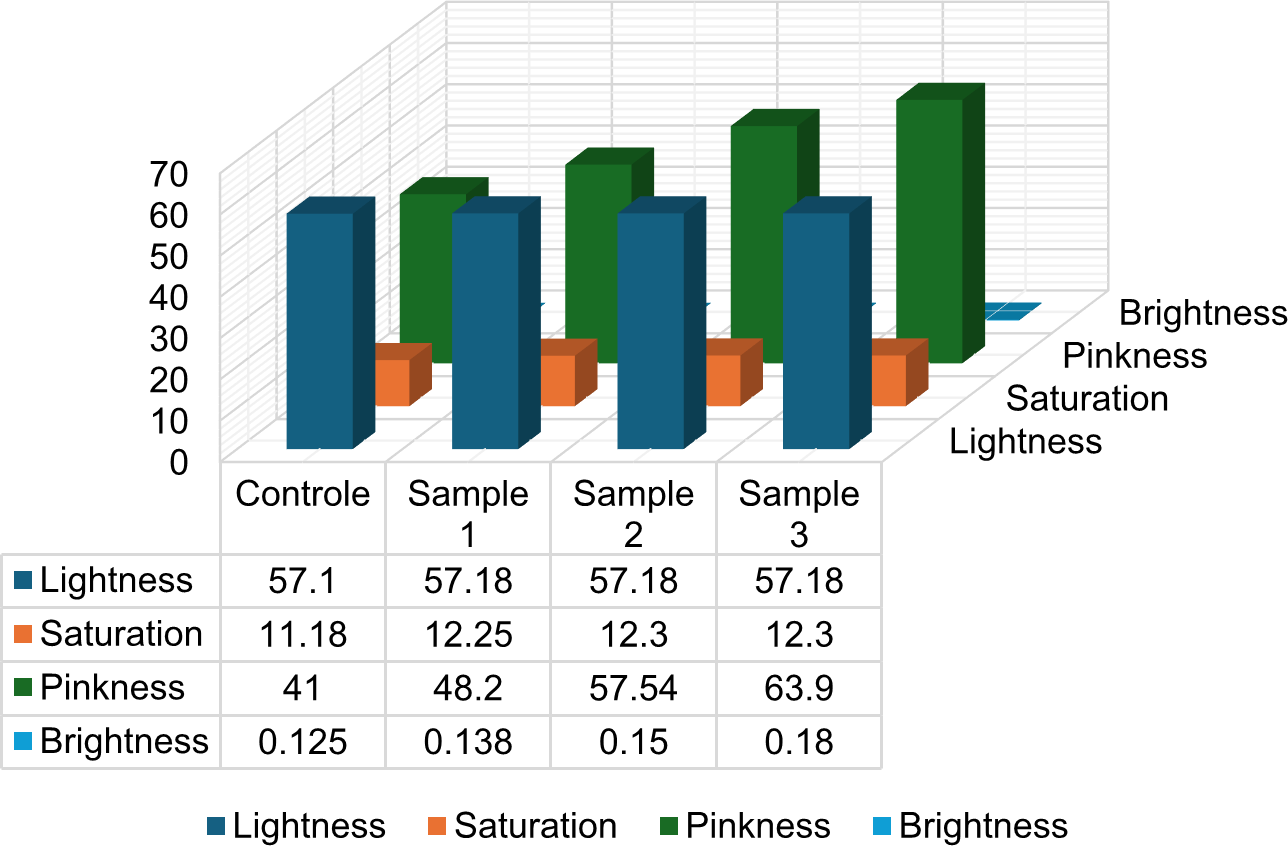
\includegraphics[width=0.6\columnwidth]{media/pish/image2}
	\caption*{Figure 2 - The result of the color characteristics of semi-smoked sausages}
\end{figure}

\begin{multicols}{2}
According to the results of Table 6, due to the primary treatment with
microorganisms at the stage of raw material preparation, we reduced the
growth of the total number of bacteria in the meat raw material, and due
to the introduction of activated starter microorganisms we obtained a
finished product with the maximum amount of the necessary microflora.

This cannot be achieved by traditional introduction of starter
microorganisms. This can be observed by comparing the indices of
mesophilic aerobic and facultative-anaerobic microorganisms between the
product sample and samples \#1, \#2, \#3. It is observed that the
microflora of sample No. 3 has increased and if the health improvement
process is not carried out properly, the microbiological indices will
increase more than normal.

This results in shortening the shelf life of the finished product. If we
consider the research after the expiry date based on Table 7, it can be
seen that the microbiological indices of the product sample are very
high. It can be seen that the finished product has not reached its shelf
life. According to the results, it can be concluded that model \#2 is
the most optimal.

The consistency of the finished samples was characterized by a more
dense, monolithic structure compared to the control, which is consistent
with the results of microstructural studies (Fig. 1). The color of
sample No. 3 was homogeneous, red. In the control, a looser consistency
was noted, the color was less intense. Thus, in sample No. 4, sour
taste, pungent odor, dark red color was detected. This may be due to the
presence of lactic acid microorganisms in the experimental sample, which
play an important role in the formation of the flavor of semi-smoked
sausages. The flavor in sample No. 3, made with propionic acid bacteria,
differs from the rest by a pronounced taste and aroma.

The data of organoleptic evaluation agree with the data of the results
of color characteristics of sausages and structural and mechanical
indicators (Fig. 2).

The performed differential analysis showed that treatment of raw
materials with propionic acid bacteria makes it possible to reduce the
lightness index and increase the rose part of the spectrum, which forms
higher levels of saturation and brightness of color of finished
products.

{\bfseries Conclusion.} The quality of finished product, pH-activity,
concentration of organic acids, microbiological quality and organoleptic
properties of semi-smoked sausage treated with liquid propionic acid
bacteria `ProBioLiz' (2 strains of propionic acid bacteria
Propionibacterium shermani and lactobacillus Lactobacillus acidophilus,
L.casei, L.Plantarum) were studied.

The optimal ratio of using liquid propionic acid bacteria `ProBioLiz' (2
strains of propionic acid bacteria Propionibacterium shermani and
lactobacillus Lactobacillus acidophilus, L.casei, L.Plantarum) is 0.1\%,
fermentation time - 8 hours.

Considering the works of the above-mentioned researchers and the results
obtained in the course of research, the technology of semi-smoked
sausage with the use of starter cultures was developed.

On the basis of the obtained data it is established that the use of
propionic acid microorganisms in the processing of meat products leads
to the disintegration of fibrous weights.

Technological scheme of production of traditional semi-smoked sausages
does not require special technical changes, so the new type of product
can be produced at any meat processing enterprise.
\end{multicols}

\begin{center}
{\bfseries References}
\end{center}

\begin{references}
1. F.Yu. Eker, H. Yardibi, O. Yesil, G. M. Bayrakal, G. Demirel Effect
of starter cultures combinations on lipolytic activity and ripening of
dry fermented sausages // Italian Journal of Animal Science. - 2014. -
Vol. 13(4). - P. 776-781. DOI 10.4081/ijas.2014.3422.

2. A.M. Ciuciu Simion, C. Vizireanu, P. Alexe, I. Franco, J. Carballo
Effect of the use of selected starter cultures on some quality, safety
and sensorial properties of Dacia sausage, a traditional Romanian
dry-sausage variety//Food Control. - 2014.- Vol.35.- P. 123-131.

DOI 10.1016/j.foodcont.2013.06.047

3. P. Nedelcheva, Z. Denkova, P. Denev, A. Slavchev, A. Krastanov
Probiotic Strain Lactobacillus \\Plantarum NBIMCC 2415 with Antioxidant
Activity as a Starter Culture in the Production of Dried Fermented Meat
Products // Biotechnology \& Biotechnological Equipment. -2014. -Vol.
24(1). -P. 1624-1630. DOI
\href{https://doi.org/10.2478/V10133-010-0016-4}{10.2478/V10133-010-0016-4}

4. I.A. Khankhalaeva, I.S. Khamagaeva, A.P. Nikiforova Effects of
propionic-acid bacteria and \\bifidobacteria on the quality of raw smoked
\emph{//}
\href{https://library.kazatu.kz:2057/sourceid/21100777291}{Foods and Raw
Materials}\emph{. -}2017. - Vol.5(1). - P. 20-29. DOI
10.21179/2308-4057-2017-1-20-29

5. M.
\href{https://library.kazatu.kz:2057/authid/detail.uri?origin=resultslist&authorId=7801545833&zone=}{Laranjo,}
M.E. Potes, M.
\href{https://library.kazatu.kz:2057/authid/detail.uri?origin=resultslist&authorId=35086070100&zone=}{Elias}
Role of starter cultures on the safety of fermented meat products //
\href{https://library.kazatu.kz:2057/sourceid/21100226442?origin=resultslist}{Frontiers
in Microbiology}. -2019. -Vol.10. DOI 10.3389/fmicb.2019.00853

6. S.E. Shukesheva,
Y.M.~\href{https://library.kazatu.kz:2057/authid/detail.uri?origin=resultslist&authorId=55968622400&zone=}{Uzakov,}
I.M. Chernukha, ~Z.S.
\href{https://library.kazatu.kz:2057/authid/detail.uri?origin=resultslist&authorId=56031451100&zone=}{Nabiyeva,}
A. Kozybayev Investigation of the influence of starter cultures on the
acceleration ripening period finished meat products //
\href{https://library.kazatu.kz:2057/sourceid/13884?origin=resultslist}{Acta
Technica CSAV (Ceskoslovensk Akademie Ved)}. -2018. - Vol. 63(1).- P.1-8
p.

7. Sirina N., Loyeau P., Ruiz M., Stegmayer M., Soto L., Werning M.,
Frizzo L. Development of probiotic fermented sausages and viability
monitoring of supplemented Lactiplantibacillus plantarum BFL strain //
Fermentation. -2022. -Vol. 8(10):526

DOI
\href{https://doi.org/10.3390/fermentation8100526}{10.3390/fermentation8100526}

8. Nie X.H., Lin S.L., Zhang Q.L. Proteolytic characterization in grass
carp sausage inoculated with Lactobacillus plantarum and Pediococcus
pento saceus. // Food Chemistry. -2014. -Vol. 145. - Р. 840--844.
\href{https://doi.org/10.1016/j.foodchem.2013.08.096}{DOI
10.1016/j.foodchem.2013.08.096.}

9. Magala M., Karovičová J., Karovičová J., Staruch L. The influence of
lactobacillus paracasei LPC- 37 on selected properties of fermented
sausages // Po- travinarstvo.- 2015. -Vol. 9(1). - Р. 58-65. DOI
\href{https://doi.org/10.5219/430}{10.5219/430}

10. TR TS {[}TR CU{]} 034/2013 O bezopasnosti myasa i myasnoj produkci
{[}On the safety of meat and meat products{]}, elektron.resurs
{[}electronic resource{]}. -2013. URL:
\href{https://docs.eaeunion.org/docs/ru-ru/0043629/cncd\_11102013\_68}{https://docs.eaeunion.org}. Date of address: 22.09.2024
\end{references}

\begin{authorinfo}
\emph{{\bfseries Information about the authors}}

Baitukenova Sh.B. - Candidate of Technical Sciences, Acting Associate
Professor, NAO `Kazakh Agrotechnical Research University named after
S.Seyfullin', Astana, Kazakhstan, e-mail:
\href{mailto:baytukenova75@mail.ru}{\nolinkurl{baytukenova75@mail.ru}};

Ryspaeva U.A. - Master' s student, Kazakh University of
Technology and Business named after K. Kulazhanov, Astana, \\Kazakhstan,
e-mail:
\href{mailto:ulzhan.ryspaeva@bk.ru}{\nolinkurl{ulzhan.ryspaeva@bk.ru}};

Baitukenova C.B. - Candidate of Technical Sciences, Associate Professor
of the Department of Technology and Standardisation, Kazakh University
of Technology and Business named after K. Kulazhanov, Astana,
Kazakhstan, e-mail:
\href{mailto:saule7272@mail.ru}{\nolinkurl{saule7272@mail.ru}}.

\emph{{\bfseries Сведения об авторах}}

Байтукенова Ш.Б.- кандидат технических наук, и.о. ассоциированного
профессора, НАО «Казахский агротехнический исследовательский университет
им. С.Сейфуллина», Астана, Казахстан, e-mail:
\href{mailto:baytukenova75@mail.ru}{\nolinkurl{baytukenova75@mail.ru}};

Рыспаева У.А. -- магистр, АО «Казахский университет технологии и бизнеса
имени К. Кулажанова», Астана, Казахстан, e-mail:
\href{mailto:ulzhan.ryspaeva@bk.ru}{\nolinkurl{ulzhan.ryspaeva@bk.ru}};

Байтукенова С.Б.-кандидат технических наук, ассоциированный профессор,
АО «Казахский университет технологии и бизнеса имени К. Кулажанова»,
Астана, Казахстан, e-mail:
\href{mailto:saule7272@mail.ru}{\nolinkurl{saule7272@mail.ru}}.
\end{authorinfo}
